\documentclass[aspectratio=169%可调屏宽比16:9(169),4:3(43)
,serif,mathserif]{beamer}
\mode<presentation>{
%\usetheme{default}
%\usetheme{AnnArbor}
%\usetheme{Antibes}
%\usetheme{Bergen}
%\usetheme{Berkeley}
%\usetheme{Berlin}
%\usetheme{Boadilla}
%\usetheme{CambridgeUS}
%\usetheme{Copenhagen}
%\usetheme{Darmstadt}
%\usetheme{Dresden}
%\usetheme{Frankfurt}
%\usetheme{Goettingen}
%\usetheme{Hannover}
%\usetheme{Ilmenau}
%\usetheme{JuanLesPins}
%\usetheme{Luebeck}
\usetheme{Madrid}
%\usetheme{Malmoe}
%\usetheme{Marburg}
%\usetheme{Montpellier}
%\usetheme{PaloAlto}
%\usetheme{Pittsburgh}
%\usetheme{Rochester}
%\usetheme{Singapore}
%\usetheme{Szeged}
%\usetheme{Warsaw}
% As well as themes, the Beamer class has a number of color themes
% for any slide theme. Uncomment each of these in turn to see how it
% changes the colors of your current slide theme.
%\usecolortheme{albatross}
%\usecolortheme{beaver}
%\usecolortheme{beetle}
%\usecolortheme{crane}
%\usecolortheme{dolphin}
%\usecolortheme{dove}
%\usecolortheme{fly}
%\usecolortheme{lily}
%\usecolortheme{orchid}
%\usecolortheme{rose}
%\usecolortheme{seagull}
%\usecolortheme{seahorse}
%\usecolortheme{whale}
%\usecolortheme{wolverine}
%\setbeamertemplate{footline} % To remove the footer line in all slides uncomment this line
%\setbeamertemplate{footline}[page number] % To replace the footer line in all slides with a simple slide count uncomment this line
%\setbeamertemplate{navigation symbols}{} % To remove the navigation symbols from the bottom of all slides uncomment this line
}
\usepackage{adjustbox}
\usepackage{hyperref}
\usepackage{indentfirst} 
\usepackage{amsmath, amsfonts, epsfig, xspace}
\usepackage{algorithm,algorithmic}
\usepackage{beamerthemesplit}
\usepackage{booktabs}
\usepackage{bm}
\usepackage{braket}
\usepackage{calligra}
\usepackage[T1]{fontenc}
\usepackage{fontspec}
\usepackage{ctex}
\usepackage{latexsym}
\usepackage{multicol}
\usepackage{multimedia}
\usepackage{calligra} \DeclareMathAlphabet{\mathcalligra}{T1}{calligra}{m}{n} \DeclareFontShape{T1}{calligra}{m}{n}{<->s*[2.2]callig15}{}
\usepackage{pstricks,pst-node}
\usepackage{ragged2e}
\usepackage{setspace}
\usepackage[normal,tight,center]{subfigure}
\setlength{\subfigcapskip}{-.5em}
\setlength{\parindent}{2em}
\begin{document}
\title{Research progress of neural network repairing} % The short title appears at the bottom of every slide, the full title is only on the title page
\author[Chi~Zhiming]{Reporter:~Chi~Zhiming} % Your name
\institute[ISCAS] % Your institution as it will appear on the bottom of every slide, may be shorthand to save space
{	
	%Lanzhou University \\ % Your institution for the title page
	%\medskip
	%\textit{chizhm16@lzu.edu.cn} % Your email address
}

	\CTEXoptions[today=old]
	\date{\today} % Date, can be changed to a custom date
\begin{frame}[plain]\vspace{1.5em}
\titlepage\vspace{-0.5cm}
%\centerline{\includegraphics[height=0.30\textheight]{logo.png}}
%\hfill 指导教师:xxx
\end{frame}
\begin{frame}{目录}
\tableofcontents
\end{frame}
\AtBeginSection[]
{
\begin{frame}{\tiny}
\frametitle{目录}
\tableofcontents[currentsection]
\end{frame}
}
%----------------------------------------------------------------------------------------
%	PRESENTATION SLIDES
%----------------------------------------------------------------------------------------

%------------------------------------------------
\section{Existing research} % Sections can be created in order to organize your presentation into discrete blocks, all sections and subsections are automatically printed in the table of contents as an overview of the talk
%------------------------------------------------
\begin{frame}
	\frametitle{Art}
	\begin{figure}[htbp]
		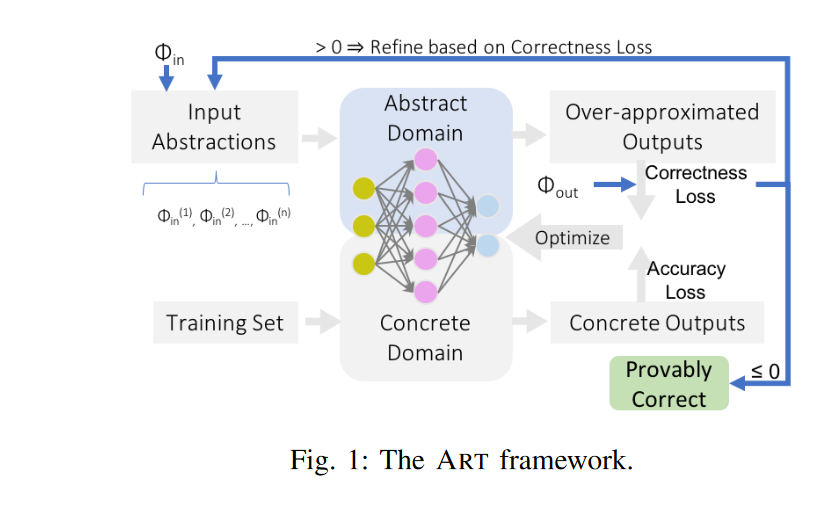
\includegraphics[width=.7\linewidth]{1.png}
	\end{figure}
\end{frame}

\begin{frame}
	\frametitle{REASSURE}
	\begin{figure}[htbp]
		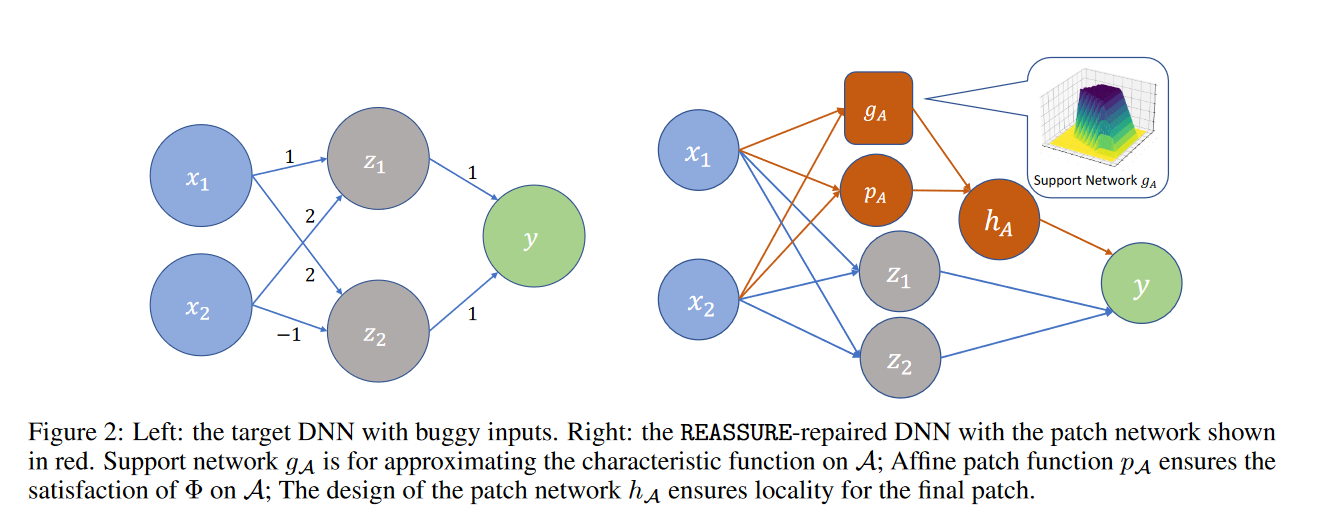
\includegraphics[width=.9\linewidth]{2.png}
	\end{figure}
\end{frame}


% Preceding work
\section{Preliminary Study}
\begin{frame}
	\frametitle{The challenging of REASSURE}
	\begin{itemize}
		\item The number of activation patterns is exponential.
		\item It can not repair the mutiple properties. 
	\end{itemize}
\end{frame}



\begin{frame}
	\frametitle{Our idea}
	\begin{itemize}
		\item Repairing regions: polytopes $\to$ regions partitioned by NN.
		\item Patch networks: linear function $\to$ NN.
		\item Framework: leverage the framework of Art to training the support network and patch network until the NN satisfy the desired properties.
	\end{itemize}
\end{frame}

\begin{frame}
	\frametitle{Current progress}
	\begin{itemize}
		\item Be familiar with the code of ART and REASSURE
		\item Encoding the support networks and patch networks to the framework of ART.
		% \item Have trained the repaird network 
	\end{itemize}
\end{frame}

\section{Future Work}
\begin{frame}
	\frametitle{Future Work}
	\begin{itemize}
		\item Construct the one-to-one correspondence between support networks and patch networks
		\item The number and framework of support networks and patch networks: hard-coding $\to$ heuristic
		\item Research the performence when we train the repaired network with fixing the original parameters of NN rather then not fix them.
		\item More properties, such as fairness and robustness.
	\end{itemize}
\end{frame}

%------------------------------------------------


%------------------------------------------------

%------------------------------------------------


%------------------------------------------------
\begin{frame}
\hfill
\center{\Huge{\calligra{\Huge{Thank you}}}}
\linespread{3}\selectfont
\end{frame}
%----------------------------------------------------------------------------------------
\end{document}